\documentclass[a4paper,10pt]{report}
\usepackage[frenchb]{babel}
\usepackage[utf8]{inputenc}
\usepackage[T1]{fontenc}
\usepackage{graphicx}
\usepackage{mathenv}
\usepackage{algpseudocode}
\usepackage{float}
\usepackage{hyperref}
\usepackage[final]{pdfpages} 
\usepackage{changepage}
\usepackage{graphicx}
 \usepackage{xcolor}

\usepackage{array}

\usepackage{caption}

\usepackage[linesnumbered,ruled]{algorithm2e}

\usepackage{amssymb}

\newcounter{cnt}
\newcommand{\definition}{
  \addtocounter{cnt}{1}
 \textbf{Définition}
}



% Title Page
\title{Université d'Angers \\  \emph{M2 Intelligence Décisionnelle \\} \hrulefill \\ \textbf{Extraction de motifs fréquents sous contraintes par approche métaheuristique} \\ \hrulefill}
\author{Ugo Rayer}


\begin{document}

    \begin{titlepage}

\newcommand{\HRule}{\rule{\linewidth}{0.5mm}}

\center 

\textsc{\LARGE Université d'Angers}\\[1.5cm] 
\textsc{\Large M2 Intelligence Décisionnelle}\\ [0.5cm] 
\textsc{\large }\\[0.5cm] 


\HRule \\[0.4cm]
{ \huge \bfseries Extraction de motifs fréquents sous contraintes par approche métaheuristique}\\[0.4cm] 
\HRule \\[1.5cm]
 

\begin{minipage}{0.4\textwidth}
\begin{flushleft} \large
\emph{Auteur:}\\
Ugo \textsc{Rayer} 
\end{flushleft}
\end{minipage}
~
\begin{minipage}{0.4\textwidth}
\begin{flushright} \large
\hfill
\begin{tabular}{@{}l@{}}
\emph{Encadrants:}\\
Benoit \textsc{Da Mota} \\
Béatrice \textsc{Duval} \\
David \textsc{Lesaint} 
\end{tabular}
\end{flushright}
\end{minipage}\\[4cm]



{\large \today}\\[3cm] 




\includegraphics{./img/ua.jpg}\\[1cm]

\vfill 

\end{titlepage}

\newpage
~
\newpage
\chapter*{Remerciements}

Avant toute chose, je tiens à remercier l'ensemble des personnes qui ont participé, de près ou de loin, à la réalisation de ce stage et à l'écriture de ce rapport. \\

\hspace{0.2cm}Des remerciements spéciaux sont adressés d'une part au Laboratoire d'Etude et de Recherche en Informatique d'Angers pour son accueil et d'autre part au projet GRIOTE de la région Pays de la Loire qui a financé cette étude. Ensuite, je tiens à remercier chaleureusement Madame Duval et Messieurs Da Mota et Lesaint pour la qualité de leur encadrement et les différentes remarques qu'ils m'ont prodiguées pendant ces quelques mois. \\

\hspace{0.2cm}Enfin, un grand merci à Josépha pour ses précieux conseils d'écriture malgré l'incompréhension générale des sujets abordés.

\tableofcontents
\newpage

\chapter{Introduction}
Le calcul des motifs fréquents est une notion essentielle dans de nombreux domaines liés à la découverte et l'extraction de connaissances. Initiallement introduit par Agrawal et al. dans \cite{AGR93}, ces motifs étaient alors utilisés pour l'établissement de règles d'associations visant à caractériser les habitudes d'achats de clients d'un supermarché. Par exemple, une règle de la forme "Pain \& Beurre $\Rightarrow$ Jambon (75\%)" signifie que 3 clients sur 4 achetant du pain et du beurre achètent également du jambon. Le calcul de telles règles se fait en deux étapes, dont la principale (i.e. disposant de la plus grosse complexité calculatoire) correspond au calcul des motifs fréquents. Depuis son introduction, le problème du calcul des motifs fréquents a été très largement étudié et appliqué à de nombreux domaines comme en bio-informatique, en cybersécurité et bien évidemment en marketing.\\

\hspace{0.15cm}L'avènement de l'ère du Big Data a fait rentrer le problème de calcul des motifs fréquents dans une nouvelle dimension. En effet, le volume de données produites dans tous les domaines a cru de manière vertigineuse ces dernières années, rendant l'extraction de connaissances d'autant plus nécessaire et délicate. De fait, la problématique du passage à l'échelle des méthodes exactes est devenue primordiale. Bien que divers efforts en ce sens aient été faits au travers de nombreuses publications, ils se concentrent généralement sur l'optimisation et la parallélisation des méthodes existantes. \\

\hspace{0.15cm}Les métaheuristiques sont des méthodes algorithmiques d'optimisation visant à résoudre des problèmes difficiles pour lesquels les méthodes exactes sont soit inexistantes soit impossibles à mettre en place en pratique. Généralement, une métaheuristique tend à faire évoluer une ou plusieurs solutions vers un optimum global en effectuant itérativement des mouvements de voisinage (légère modification) sur la solution courante. De nombreuses métaheuristiques ont été proposées et largement appliquées à de nombreux problèmes, allant de la simple recherche locale aux algorithmes mémétiques offrant une combinaison entre algorithme génétique et recherche locale. \\

\hspace{0.15cm}Ainsi, nous formaliserons le problème de calcul de motifs fréquents sous contraintes dans le chapitre suivant avant d'effectuer un état de l'art des méthodes existantes. Le chapitre 4 sera dédié à la présentation de nos contributions dont nous discuterons des résultats en section 5. Le dernier chapitre sera consacré à la conclusion de cette étude et à une ouverture vers de futurs travaux.

\newpage
\chapter{Le problème du calcul des motifs fréquents}

\section{Définition du problème}
	Ce problème a été largement étudié au travers de différentes théories. La première et principale est la théorie des ensembles et treillis sur laquelle la présentation du problème sera faite. Nous pouvons également noter que ce problème a été abordé par la théorie des graphes. En effet, le problème d'extraction de motifs fréquents peut se voir comme le calcul d'une clique maximale au sein d'un graphe bipartite. Dans un premier temps, noud poserons un cadre formel nécessaire à la définition du problème que nous illustrerons ensuite. Dans un second temps, nous introduirons quelques propriétés dérivées de la définition du problème et utilisées par de nombreuses méthodes exactes.

\subsection{Formalisation}
	Soit $\mathcal{I}$ un ensemble de \emph{symboles} appelées \textbf{items}. Quelque soit \emph{I} $ \subseteq \mathcal{I}$, \emph{I} est un \emph{motif} appelé \textbf{itemset}. \\

\hspace{0.15cm}Soit $\mathcal{T}$ = \{ \emph{$t_{1}$, ... , $t_{n}$ } \} un ensemble de \textbf{transactions}. Chaque élément \emph{$t_{i}$} est un couple $< tid, \emph{I} >$ où \emph{tid} est l'identifiant de la transaction et \emph{I} $\subseteq \mathcal{I}$. $\mathcal{T}$ est communément appelé \textbf{base de transactions}.  \\

\hspace{0.15cm}Pour tout itemset \emph{I} $\subseteq \mathcal{I}$ la \textbf{couverture} de \emph{I} par $\mathcal{T}$ est définie par : \\
\begin{center}
\textbf{cover$_{\mathcal{T}}$}(\emph{I}) = \{ \emph{t} $\in \mathcal{T}  | \emph{ I} \subseteq \emph{t }\}$
\end{center}

\hspace{0.15cm}La cardinalité de la couverture d'un itemset \emph{I} par $\mathcal{T}$ \\
\begin{center}
\textbf{sup$_{\mathcal{T}}$}(\emph{I}) = $|$ \textbf{cover$_{\mathcal{T}}$}(\emph{I}) $|$
\end{center}
est appelée \textbf{support} de \emph{I}.  Etant donné un support minimal \emph{minsup} l'ensemble des \textbf{itemsets} (i.e. motifs) \textbf{fréquents} est défini par : \\
\begin{center}
$\textbf{F}_{\mathcal{T},minsup}$ = \{ \emph{I} $\subseteq \mathcal{I } |$  $sup_{\mathcal{T}}(\emph{I}) \geq$ \emph{minsup} \}
\end{center}

\hspace{0.15cm}Le problème du \textbf{calcul des itemsets fréquents} ( \textbf{FIM} - \emph{Frequent Itemsets Mining}) est, étant donné une base de transactions $\mathcal{T}$ et un support minimal \emph{minsup} de calculer l'ensemble \emph{F} des itemsets fréquents. Comme F. Boden le remarque dans \cite{BOD06}, bien qu'historiquement définie comme une valeur relative et donc asujettie à un support minimal défini dans l'intervalle [0,1], le support est de nos jours mesuré de manière absolue. Si nécessaire, nous y ferons référence sous la notion de fréquence : \\
\begin{center}
$\textbf{Freq}_{\mathcal{T}}$(\emph{I}) = $\frac{ | \textbf{ cover$_{\mathcal{T}}$}(\emph{I})  | } { | \mathcal{T} | }$
\end{center}
avec \emph{minfreq} simplement définie par $\frac{\emph{minsup}}{| \mathcal{T} |}$. \\

\subsection{Exemple}
	Situons nous dans le contexte de la définition historique de problème et considérons la base de transactions suivante. Le tableau 1 décrit chaque transaction par : un identifiant, une liste d'objets achetés et la liste des items fréquents vis à vis d'un support minimal de  3.\\

\begin{tabular}{|c|l|l|}
	\hline
	ID transaction & Objets achetés & Items Fréquents Ordonnés \\
	\hline
	100 & f, c, a, d, g, i m, p & f, c, a, m, p \\
	\hline
	200 & a, b, c, f, l, m, o & f, c, a, b, m \\
	\hline
	300 & b, f, h, j, o & f, b \\
	\hline
	400 & b, c, k, s, p & c, b, p \\
	\hline
	500 & a, f, c, e, l, p, m, n & f, c, a, m, p \\
	\hline	
\end{tabular}
\captionof{table}{Base de transactions exemple}
\vspace{0.4cm}

\hspace{0.15cm}Une fois calculé, l'ensemble des itemsets fréquents vis à vis de ce jeu de données $\mathcal{T}$ est l'ensemble $\textbf{F}_{\mathcal{T},3}$ = \{ (f:4), (c:4), (a:3), (b:3), (m:3), (p:3), (fc:3), (fa:3), (fm:3), (cm:3), (cp:3), (ca:3), (am:3), (fca:3), (fcm:3), (fam:3), (cam:3), (fcam:3) \}.  \\

\subsection{Complexité et Propriétés}
La complexité du problème vient d'une part du nombre d'itemsets à considérer en fonction du nombre d'objets et d'autre part de nombre de transactions dans la base. En effet, soit \emph{n} objets fréquents dans la base, il y a alors $2^{n}$ itemsets possibles. D'autre part, le calcul du support d'un itemset se fait au travers de l'ensemble des transactions. L'efficacité d'une méthode à résoudre ce problème se fera donc par sa capacité à explorer intelligement l'espace des $2^{n}$ itemsets et par son efficacité à calculer le support d'un itemset vis à vis de $| \mathcal{T} |$. \\
\hspace{0.15cm}Différents théorèmes et propriétés issus de l'étude de ce problème sont utilisés dans les méthodes proposées pour le résoudre. Nous présentons les propriétés liées à la monotonie du support d'un ensemble et renvoyons le lecteur vers \cite{BOD06} et \cite{GOE} pour plus de détails. \\
\textbf{Monotonie du support.} Soit une base de transactions $ \mathcal{T} sur \mathcal{I} $ et soient \emph{X, Y} $\subseteq \mathcal{I}$ deux itemsets. Alors, \\
\begin{center}
\emph{X} $\subseteq $ \emph{Y} $\Rightarrow$ \textbf{sup$_{\mathcal{T}}$}(\emph{Y}) $ \leq $ \textbf{sup$_{\mathcal{T}}$}(\emph{X})
\end{center}

Cette propriété nous permet de dire que si un k-itemset \emph{X} (i.e. un itemset comprenant k objets) est fréquent, alors l'ensemble \emph{Y} des k-1-itemsets $\subset $\emph{X} est fréquent. Par exemple, (fca:3) est fréquent, de même que (fc:3), (fa:3) et (ca:3). \\
Nous pouvons de manière duale dire que si un k- itemset \emph{X} est non-fréquent, alors aucun des k+1-itemset \emph{Y} tel que \emph{X} $ \subset $ \emph{Y} n'est fréquent. Ces deux observations sont à la base des différents sens de parcours de l'espace de recherche des $2^{n}$ itemsets possibles dans la plupart des algorithmes.

\section{Itemsets clos \& maximaux}

\hspace{1.5cm}Afin de réduire l'espace de recherche, il a été proposé de contraindre la recherche à l'ensemble des itemsets clos. Un k-itemset \emph{X} fréquent est clos si \textbf{sup$_{\mathcal{T}}$}(\emph{X}) $>$ \textbf{sup$_{\mathcal{T}}$}(\emph{Y}) $ \forall  $ \emph{Y} tel que \emph{X} $ \subset $ \emph{Y}.  Littéralement, un itemset est clos si son support décroit lorsqu'il est étendu. \\

\hspace{1.5cm}Un itemset clos est maximal si aucun de ses surensembles n'est fréquent. Formellement, un k-itemset \emph{X} est maximal si \textbf{sup$_{\mathcal{T}}$}(\emph{X}) $>$ \textbf{sup$_{\mathcal{T}}$}(\emph{Y}) $\forall \emph{Y}  | \emph{X} \subset \emph{Y}$. \\

\hspace{1.5cm}Ainsi dans notre exemple, l'ensemble des itemsets clos est   $\textbf{C}_{\mathcal{T},3}$ = \{ (f:4), (c:4), (b:3), (cp:3), (fcam:3) \} et l'ensemble des itemsets clos maximaux est  $\textbf{MC}_{\mathcal{T},3}$ =  $\textbf{C}_{\mathcal{T},3} - $ \{ (f:4), (c:4) \}. La figure suivante représente le treillis complet des différents itemsets possibles sur les objets fréquents. Y figurent d'une part les itemsets fréquents en vert, d'autre part les itemsets clos en jaune et enfin les itemsets maximaux en rouge. Pour plus de lisibilité, les itemsets non-fréquents ne figurent pas dans le treillis.\\

\begin{figure}
	\begin{adjustwidth}{-2.7cm}{}
	\begin{tabular}{l}
	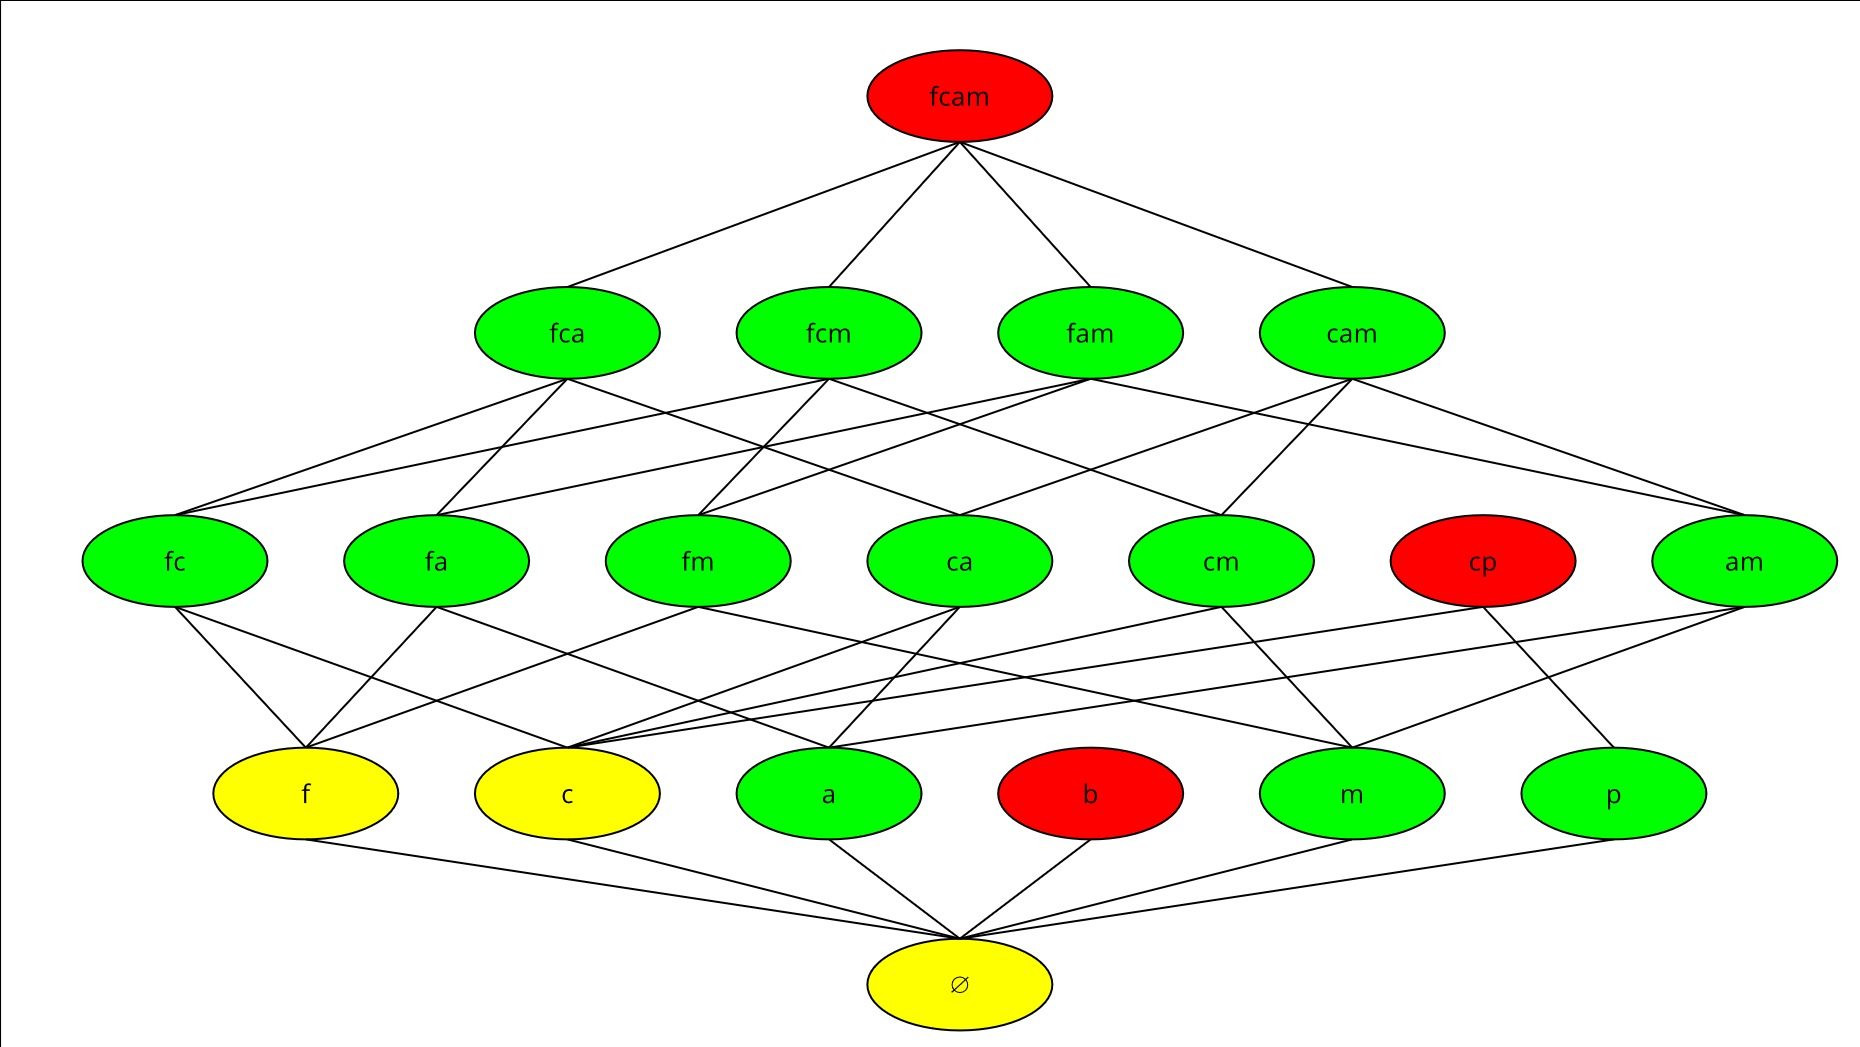
\includegraphics[width=12cm,height=10cm]{./img/treillis_is.jpg}\\
	\end{tabular}
	\caption{\label{fig:text}Treillis des itemsets \textcolor{green}{fréquents}, \textcolor{yellow}{clos} et \textcolor{red}{maximaux} de notre exemple}
	\end{adjustwidth}
\end{figure}

Zaki et al. et Pas. et al. prouvent dans \cite{ZAK99} et \cite{PAS99} que l'intégralité des itemsets fréquents peut être dérivée de l'ensemble des itemsets clos et/ou maximaux. Ils proposent alors d'adapter les méthodes existantes pour le calcul des itemsets clos maximaux.  

\newpage

\section{Itemset et classification}

	Dans cette section nous redéfinissons le problème à considérer permettant l'usage raisonnable de méthodes heuristiques pour le résoudre. Nous l'aborderons dans un premier temps sous l'aspect d'un problème combinatoire solvable par recherche locale. Ensuite, nous proposerons une recherche itérée avec ses avantages avant d'envisager une approche évolutionnaire. \\

\subsection{Définition du problème}
	Sortant d'un contexte d'extraction de motifs fréquents pour l'établissement de règles d'associations, nous nous plaçons maintenant dans un contexte de classification binaire d'un ensemble de transactions. Notre objectif reste cependant d'avoir une approche généraliste, i.e. sans disposer d'informations du contexte d'application des méthodes proposées. \\ 
	Soit $\mathcal{T}$ une base de transactions définie sur $\mathcal{N}$ items. En plus d'un identifiant et de ses items, chaque transaction possède une classe (positive ou négative). A partir de là, le but du problème est de trouver un itemset X offrant la meilleure classification possible. Cependant, la difficulté résulte maintenant dans la mesure à adopter pour évaluer la qualité d'une solution. Pour appréhender cette difficulté, le tableau suivant récapitule les 4 ensembles de bases à déterminer pour une solution vis à vis de $\mathcal{T}$. \\

\begin{center}
	\begin{tabular}{|c|c|c|}
		\hline
		& $\emph{S} \subseteq \emph{t}$ & $\emph{S} \not\subseteq \emph{t}$ \\
		\hline
		Classe \emph{t} = 1 & $\emph{t} \in TP$ & $\emph{t} \in FP$ \\
		\hline
		Classe \emph{t} = 0 & $\emph{t} \in FN$ & $\emph{t} \in TN$ \\
		\hline
	\end{tabular}
\end{center}





\subsection{Représentation et évaluation d'une solution}

	Le problème étant de trouver un itemset maximisant la couverture de la classe positive tout en minimisant son support dans la classe négative, une solution du problème est simplement un bitset \emph{S} de $\mathcal{N}$ bits tel que $\forall \emph{i} \in [1..\mathcal{N}] \emph{S}_{i} = 1$ si l'item \emph{i} appartient à la solution, $\emph{S}_{i}$ = 0 sinon. \\
	L'évaluation d'une solution doit permettre de quantifier la corrélation des différents items dans leur pouvoir de classification de la base de transactions. Diverses mesures existent et ont été proposées et largement étudiées dans la littérature (citation TAN02, GEN06, ...).\\
	Dans une problématique de classification, de nombreuses mesures sont basées sur les 4 ensembles décrivant la matrice de confusion des performances d'un classifieur :
\begin{center}
	- Vrai positif (TP) : $\forall \emph{i} \in [1..\mathcal{N}]$  $\emph{S}_{i} = 1 et \emph{t}_{i} = 1$ \&  $\emph{t} \in C^{+}$ \\
	- Faux Positif (FP) : $\exists \emph{i} \in [1..\mathcal{N}]$ tel que $\emph{S}_{i} = 1, \emph{t}_{i} = 0$ \&  $\emph{t} \in C^{+}$\\
	- Vrai Négatif (TN) : $\exists \emph{i} \in [1..\mathcal{N}]$ tel que $\emph{S}_{i} = 1, \emph{t}_{i} = 0$ \&  $\emph{t} \in C^{-}$\\
	- Faux Négatif (FN) : $\forall \emph{i} \in [1..\mathcal{N}]$ $\emph{S}_{i} = 1, \emph{t}_{i} = 1$ \&  $\emph{t} \in C^{-}$\\
\end{center}

 Le tableau suivant récapitule l'appartenance d'une transaction \emph{t} à un des quatre ensembles : 
	 

La précision d'une telle classification correspond au rapport entre le nombre de réponses pertinentes données (TP) et le nombre de réponses données (TP+FP). Le rappel correspond quant à lui au rapport entre le nombre de réponses pertinentes données (TP) et le nombre de réponses pertinantes existant (TP+FN). 

\begin{center}
- Precision = $\frac{TP}{TP+FP}$ \\
\vspace{0.15cm}
- Rappel = $\frac{TP}{TP+FN}$\\
\end{center}

La \emph{F Mesure} permet d'aggréger rappel et précision en accordant un poids équivalent à chaque mesure. Cette une version simplifié de la \emph{$F_{\beta}$ Mesure} définie par la relation suivante : 
\begin{center}
- \emph{$F_{\beta}$} = (1+$\beta^{2}$) * $\frac{Precision*Rappel}{\beta^{2}*Precision + Rappel}$
\end{center}

Dans notre cas, où rappel et précision sont équitablement pondérés, la mesure peut se simplifier comme suit :

\begin{center}
- \emph{$F_{1}$} = $\frac{2*TP}{2*TP + FN + FP }$
\end{center}

Toutefois, cette mesure ne permet pas d'introduire les deux seuils définissant les contraintes de notre problème. De plus, le problème que nous tentons de résoudre peut être vu comme un problème d'optimisation sous contraintes et donc défini comme suit : \\

\begin{center}
	Maximize $\sum{(X_{i} = 1})$ $\forall \emph{i} \in \mathcal{I}$ s.c. \\
	$TP(X) \geq \emph{minsup}$ \\
	$FN(X) \leq \emph{maxsup}$
\end{center}

Enfin, comme le rappellent C. Dhaenens et L. Jourdan dans \emph{Metaheuristics for Big Data}, le choix dans la mesure de qualité est fortement corrélée au contexte d'application et peut donc être utilisée comme fonction objectif par une méthode d'optimisation. Dans ce sens et traitant le problème d'un point de vue générique, nous proposons donc d'évaluer une solution \emph{X} de \emph{k} items de manière générique en aggrégeant simplement notre objectif avec nos deux contraintes équitablement pondérées via la formule suivante :

\begin{center}
	$\mathcal{F}$(\emph{X}) = $\emph{k}* ( \frac{1}{2}*\frac{TP}{\emph{minsup}} + \frac{1}{2}*\frac{maxsup}{FN}$ )\\
\end{center}

Le calcul de cette évaluation nécessite un scan complet du jeux de données afin de calculer la cardinalité des ensembles TP et FN intervenant dans la fonction $\mathcal{F}$. Nous verrons ensuite que nous pourrons profiter de ce scan pour la définition du voisinage.

\subsection{Relation de voisinage}

	Après avoir défini la fonction d'évaluation d'un individu, il est nécessaire pour pouvoir mettre en place ni'mporte quel mécanisme de recherche de définir la relation de voisinage qui va nous permettre de nous déplacer au sein de l'espace de recherche. Différents points sont à considérer pour la définition d'un voisinage pertinent. En premier lieu, il est important de noter qu'il est difficile de défnir un voisinage pertinent dans le cadre d'une approche de type générique (sans information du contexte). Ensuite, en raison de la complexité de la méthode d'évaluation (nécessitant un scan complet du jeu de données) il est important de considérer la taille du voisinage comme un facteur important. En effet, un voisinage trop grand engendrera un coût calculatoire trop important et par conséquent une baisse de performance, alors qu'un voisinage trop petit ne permettra pas un déplacement efficace dans l'espace de recherche.\\
	
	Pour l'ensemble de ces raisons et pour ne pas bloquer sur une relation de voisinage informée, nous nous contenterons pour l'instant d'utiliser un voisinage simple et relativement restreint. De fait, une solution \emph{S'} appartiendra au voisinage de la solution courante \emph{S} s'il est différent de \emph{S} à un item prêt. Formellement, le voisinage d'une solution est défini comme suit : \\

\begin{center}
	$\mathcal{N}(\emph{S})$ = \{\emph{S'} tq |\emph{S'}| = |\emph{S}|+1 et $\forall \emph{i} \in \emph{S}, \emph{i} \in \emph{S'} $ \} $\cup$ \{\emph{S'} tq |\emph{S'}| = |S|-1 et $ \forall \emph{i} \in \emph{S'}, \emph{i} \in \emph{S}$\}   \\
\end{center}	

Ce voisinage est de taille fixe égale à la taille de $\mathcal{I}$. En effet, chaque item a soit la possibilité d'être ajouté ou bien d'être enlevé de la solution courante. Nous pourrons éventuellement contraindre plus spécifiquement ce voisinage en tentant de spécifier les items pouvant être ajoutés/supprimés en fonction d'informations extraites lors de l'évaluation de la solution courante.

\
\begin{center}
	\begin{tabular}{|c|c|c|c|c|c|c|}
		\hline
		\emph{tid} & A & B & C & D & E & Classe \\
		\hline
		1 & 1 & 0 & 1 & 1 & 0 & \textcolor{green}{+}\\
		\hline
		2 & 0 & 1 & 1 & 0 & 1 & \textcolor{green}{+}\\
		\hline
		3 & 1 & 0 & 1 & 1 & 0 & \textcolor{green}{+}\\
		\hline
		4 & 1 & 0 & 1 & 1 & 1 & \textcolor{green}{+}\\
		\hline
		5 & 0 & 1 & 0 & 0 & 1 & \textcolor{red}{-}\\
		\hline
		6 & 1 & 0 & 1 & 1 & 0 & \textcolor{red}{-}\\
		\hline
		7 & 0 & 1 & 1 & 0 & 1 & \textcolor{red}{-}\\	
		\hline
		8 & 1 & 0 & 0 & 1 & 1 & \textcolor{red}{-}\\	
		\hline		
	\end{tabular}
\end{center}

\end{document}